\chapter{Methods}\label{ch:methods}
This chapter aims to explain fundamentals, used in the experiments.
The focus is on the \textit{probability density function}, \textit{Boltzmann transport equation} and \textit{Lattice Boltzmann scheme}.
The combination of those principles allows simulating fluids in the experiments.
All information in this article is from the lecture of the corresponding course under Prof. Greiner at the University of Freiburg \cite{lecture}.


\section{Probability Density Function (PDF)}\label{sec:probability-density-function-(pdf)}
The Probability Density Function (PDF) is a concept that describes the probability of finding a particle at a certain position.
In theory, the simulation would need to track the individual trajectories of every particle in phase space.
This would require solving a very large number of equations.
Because solving these equations would be too costly, only the averages over the volumes in the phase space are taken using the PDF\@.
Therefore, the PDF, denoted as \(f(\mathbf r_i,\mathbf v_i,t)\), represents the probability density of finding a particle at a certain position \(\mathbf{r_i}\) and velocity \(\mathbf{v_i}\) at a given time \(t\).


\section{Boltzmann Transport Equation (BTE)}
The Boltzmann transport equation formulates the evolution of motion of the PDF over time.
It consists of two parts.
The first part is \textit{streaming} and resembles only the free movement of particles.
The second part is called \textit{collision} and deals with the interaction between particles while moving.
The whole Boltzmann Transport Equation is denoted as
\begin{equation}
    \frac{\partial f\left(\mathbf{r},\mathbf{v},t\right)}{\partial t}+\mathbf{v}\nabla_{\mathbf{r}} f\left(\mathbf{r},\mathbf{v},t\right)
    +\mathbf{a}\nabla_{\mathbf{v}} f\left(\mathbf{r},\mathbf{v},t\right)=C(f)
    \cdot
    \label{eq:bte}
\end{equation}

\subsection{Streaming}\label{subsec:streaming}
The l.h.s.\ of \cref{eq:bte} denotes the streaming part.
The streaming describes the free movement of the densities at a certain velocity.
In the context of this project, movement may happen in 2d space in 9 directions, similar to a queen in chess.
Further information is in \cref{sec:lattice-bolzmann-scheme}.

\subsection{Collision}\label{subsec:collision}
Only applying streaming resembles a 0\% probability of collision between particles, which is not realistic.
To account for collisions, an additional term is introduced at the r.h.s. of \cref{eq:bte} to represent the collision process that occurs at each time step.
In reality, collisions between particles result in an almost instantaneous exchange of energy and momentum.
However, these collisions occur in extremely short time intervals on the order of femtoseconds (\(10^{-15}\) seconds), making it impractical to measure them directly in the model.
Therefore, the collision process is approximated as an instantaneous process.
Because of this instantaneous, it cannot be represented as a differential equation, which normally describes continuous changes.
Instead, a probabilistic approach is taken to describe the effects of collisions.
\newline

The collision part of the Boltzmann transport equation was introduced on the r.h.s.\ in \cref{eq:bte}.
To simplify this collision term, a relaxation time approximation is commonly used.
This approximation assumes that the probability density function (PDF) \(f\left(\mathbf{r},\mathbf{v},t\right)\) relaxes towards a local equilibrium distribution, denoted as \(f^{eq}\left(\mathbf{r},\mathbf{v},t\right)\).
By interpreting the streaming term as the total time derivative of the PDF, the BTE can be reformulated as follows:

\begin{equation}
    \frac{d}{dt} f\left(\mathbf{r},\mathbf{v},t\right) = -\frac{ f\left(\mathbf{r},\mathbf{v},t\right)- f^{eq}\left(\mathbf{r},\mathbf{v},t\right)}{\tau}
    \cdot
    \label{eq:bgk}
\end{equation}

The included equilibirum function can be denoted as
\begin{equation}
    f_i^{eq}(\rho(\mathbf{r}),\mathbf{u}(\mathbf{r}))
    =w_i\rho(\mathbf{r})
    \left[
        1+3\mathbf{c}_i\cdot\mathbf{u}(\mathbf{r})
        +\frac{9}{2}\left(\mathbf{c}_i\cdot\mathbf{u}(\mathbf{r})\right)^2
        -\frac{3}{2}|\mathbf{u}(\mathbf{r})|^2
        \right]
    \cdot
    \label{eq:feq}
\end{equation}

The equilibrium function introduces some additional quantities, namely the density \(\rho(\mathbf{r})\), velocity \(\mathbf{u}(\mathbf{r})\) and \(w_i\).
\(w_i\) is defined for a D2Q9 lattice as seen in~\cref{eq:w}.
The other two quantities can be calculated using the following formulas
\begin{equation}
    w_i = \left(\dfrac{4}{9},
    \dfrac{1}{9}, \dfrac{1}{9}, \dfrac{1}{9}, \dfrac{1}{9},
    \dfrac{1}{36}, \dfrac{1}{36}, \dfrac{1}{36}, \dfrac{1}{36}\right)
    \label{eq:w}
\end{equation}
\begin{equation}
    \rho(\mathbf{r})=\sum_i f_i
    \label{eq:rho}
\end{equation}
\begin{equation}
    \mathbf{u}(\mathbf{r})=
    \frac{1}{\rho(\mathbf{r})}\sum_i \mathbf{c}_i f_i(\mathbf{r}) \cdot
    \label{eq:u}
\end{equation}


\section{Lattice Bolzmann Scheme}\label{sec:lattice-bolzmann-scheme}

In order to discretize the Boltzmann Transport Equation (BTE), it is necessary to incorporate both velocity and position space into the discrete scheme representation.
An effective approach involves utilizing a 2D grid, as illustrated in \cref{fig:bte-scheme}.
The grid represents the position space as coordinates of the x and y coordinates.

\begin{figure}[H]
    \begin{center}
        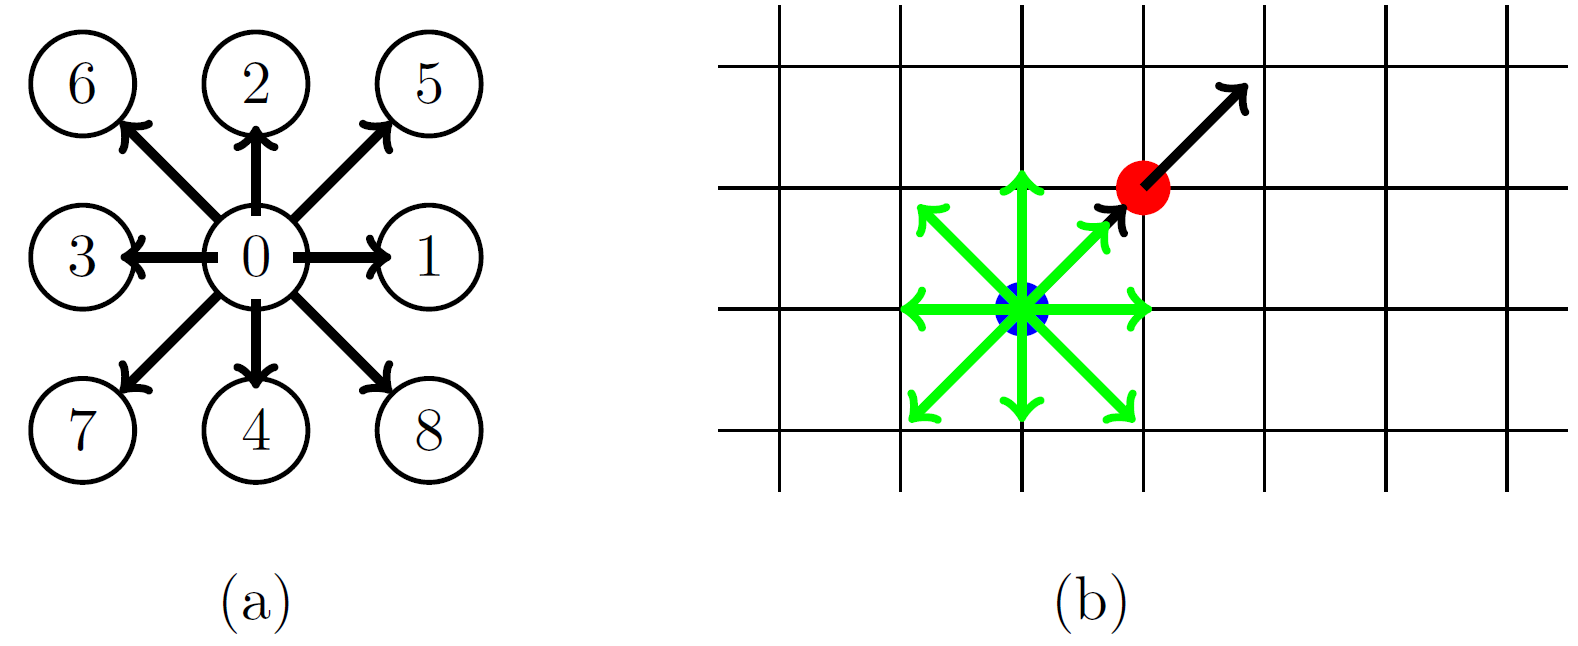
\includegraphics[width=10cm]{logos/Gitter_LBM.png}
        \caption[Visualization of the underlying grid including labled directions.]{
            Visualization of the underlying grid including labled directions. \\
            (a) directions with given labels \\
            (b) streaming example of one particle
        }
        \label{fig:bte-scheme}
    \end{center}
\end{figure}

Each position holds a probability density value, resembled by the value at that point.
The velocities are included when introducing a third dimension, that separates the different streaming directions.
To get the probability density function back, only the sum of all different directions in one point is needed.
The probability density function can be reconstructed by simply summing the values for all different directions at a given point.
\newline

The streaming, as explained in \cref{subsec:streaming}, is applied by moving the values of the points in one of 9 directions in their respective dimension.
The collision process can be implemented by employing the functions described in \cref{subsec:collision}.
During collisions, densities may be transferred between different dimensions within the scheme.


\section{Reynolds Number}\label{sec:reynolds-number}
The Reynolds Number is used to compare results of different simulations.
The same Reynolds Number indicates, that the simulations are comparable.
It is calculated by the following formula where $L$ is the size of one simulation dimension, $u$ the velocity or speed and $\nu$ the viscosity of the simulated fluid

\begin{equation*}
    \begin{gathered}
        u = avg(\sqrt{\mathbf u_x^2 * \mathbf u_y^2}) \\
        Re = \frac{L u}{\nu} \cdot
    \end{gathered}
\end{equation*}

